\chapter{Capturing a Light Field}

\section{The Plenoptic Function and the Light Field}

The plenoptic function, as introduced by~\cite{AdelsonBergen}, is a 7D function that describes the intensity of light for every frequency, along every light ray in space, at any time. 
It is defined as
\begin{align*}
	P \colon \mathbb{R}^3 \times \left[0, 2 \pi \right) \times \left[ 0, \pi \right] \times \mathbb{R}^2 & \to \mathbb{R}^+ \\
	\left(x, y, z, \theta, \phi, t, \lambda \right) & \mapsto P\left(x, y, z, \theta, \phi, t, \lambda \right), 
\end{align*}
where the parameters $\left(x, y, z\right)$ are the coordinates of a point in 3D space and the angles $\left(\theta, \phi \right)$ describe the direction of an incoming light ray at time $t$. 
The light's intensity is given for every wavelength $\lambda$ and thus, the plenoptic function not only captures the visible frequency spectrum but all electromagnetic waves. 
A commonly used measure for light is the radiance, which is obtained from P by integrating over all wavelengths: 
$R\left(x, y, z, \theta, \phi, t\right) = \int_{\mathbb{R}} \! P\left(x, y, z, \theta, \phi, t, \lambda \right) \, \mathrm{d} \lambda$.

In practice, it is impossible to acquire all the data needed to model the 7D plenoptic function and hence it is reasonable to consider only a subset of the parameters. 
Dropping the time parameter $t$ in $R\left( x, y, z, \theta, \phi, t \right) $ yields a 5D function for the radiance in a static scene. 
As described by~\cite{LightFieldRendering}, this five dimensional representation can further be reduced to four dimensions in the following way. 
The radiance along a line is constant in free space and so, the 5D plenoptic function holds redundant information for the points on this line. 
Ignoring this redundancy leads to the equivalent 4D parameterization of the ray space. 
\cite{LightFieldRendering} propose a parameterization by two parallel planes, as seen in figure~\ref{fig:LightFieldParametrization}, where the coordinates of the lines (rays) are given by the intersections with the two planes.
The \textbf{4D light field} $L(u, v, s, t)$ is therefore defined as the radiance along the line intersecting the two planes at coordinates $(u, v)$ and $(s, t)$.
This two-plane parameterization of the light field is the most common one seen in literature, but there are many ways to choose a parameterization.
For instance, one can use a plane and two angles to define each ray passing this plane, which would result in a light field $L(u, v, \theta, \phi)$ where $\theta, \phi \in (0, \pi)$.

\begin{figure}
	\centering
	\documentclass{standalone}
\usepackage{tikz}

\begin{document}
	
	\begin{tikzpicture}[scale = 0.4]
	
		\filldraw[draw = black, fill = white] (0, 0) -- (5, -2) -- (5, 5) -- (0, 7) -- cycle;
		\filldraw[draw = black, fill = white] (9, 3) -- (14, 1) -- (14, 8) -- (9, 10) -- cycle;
		
		\draw[<-] (-3, 4) -- (1, 4);
		\draw (5, 4) -- (11, 4);
		\draw (14, 4) -- (17, 4);
		
		\node [left] at (-3, 4) {$L(u, v, s, t)$};
		
		
		\draw[fill] (1, 4) circle [radius = 0.1];
		\draw[fill] (11, 4) circle [radius = 0.1];
		
		\node[below right] at (1, 4) {$(u, v)$};
		\node[below right] at (11, 4) {$(s, t)$};
	
	\end{tikzpicture}
	
\end{document}
	\caption{Parametrization of the light field with two planes.}
	\label{fig:LightFieldParametrization}
\end{figure}

\section{Light Field Acquisition}
% Figure epipolar image
% Explain epipolar images: line slope <-> depth

For practical applications, the light field must be discretized and so an appropriate sampling method needs to be chosen.
One way is to capture the light field with a grid of optical systems, e.g. cameras.
Typically, the $(u, v)$-plane is sampled on a grid $G_{uv} = \left \{ \left( u_i, v_j \right) \mid i = 1,\dots, n, j = 1, \dots, m\right \}$ on the $(u, v)$-plane with a resolution $n \times m$.
The extent in horizontal (vertical) direction is called the horizontal (vertical) \textbf{baseline}.
This means that only a slice of the actual light field can be captured and the two planes are clipped to form a rectangle.

%There are different methods to sample a light field. In principle, every camera can be used to capture 

%The samples on the $(u, v)$-plane correspond to the virtual positions of the camera. 
%Properties of the light field do not change under re-parameterization. 

\subsection*{Oblique Projection}
% Parameterization, Advantages, Disadvantages
% Mention Tomography
% Rotation 

Oblique projection, as shown in figure~\ref{fig:ObliqueProjection}, is a special case of orthographic projection: The parallel rays do not need to be perpendicular to the image plane of the camera.
The advantage is that there is a one-to-one correspondence between camera position and ray angle, since all rays in one camera are parallel.
This means that the angular resolution is simply the number of cameras, and the spatial resolution is the number of pixels in the image plane.
Given a light field $L(u, v, s, t)$ and the distance $d$ between the two planes, a re-parameterization $L^{\prime}(\theta, \phi, s, t)$ can be obtained according to figure~\ref{fig:ObliqueProjectionReparameterization} by the transformation
\begin{align*}
		& \theta = \arctan\left(\frac{u - s}{d}\right), & \phi = \arctan\left(\frac{v - t}{d}\right).
\end{align*}
However, this type of projection is only applicable for synthetic scenes that are rendered with a computer.
% TODO: Refer to a figure with a synthetic scene.

\begin{figure}[tb]
	\subfigure[]{
		\centering
		\documentclass{standalone}
\usepackage{tikz}

\begin{document}

	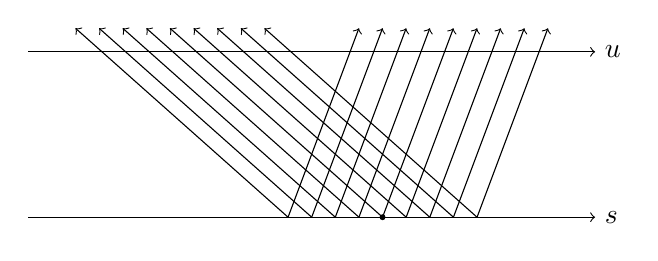
\begin{tikzpicture}[scale = 0.3, baseline]
	
		\draw[->] (-11, 0) -- (13, 0);
		\draw[->] (-11, 7) -- (13, 7);
		
		\node[right] at (13, 0) {$s$}; 
		\node[right] at (13, 7) {$u$}; 
		
		\draw[->] (0, 0) -- (-9, 8);
		\draw[->] (1, 0) -- (-8, 8);
		\draw[->] (2, 0) -- (-7, 8);
		\draw[->] (3, 0) -- (-6, 8);
		\draw[->] (4, 0) -- (-5, 8);
		\draw[->] (5, 0) -- (-4, 8);
		\draw[->] (6, 0) -- (-3, 8);
		\draw[->] (7, 0) -- (-2, 8);
		\draw[->] (8, 0) -- (-1, 8);
		
		\draw[->] (0, 0) -- (3, 8);
		\draw[->] (1, 0) -- (4, 8);
		\draw[->] (2, 0) -- (5, 8);
		\draw[->] (3, 0) -- (6, 8);
		\draw[->] (4, 0) -- (7, 8);
		\draw[->] (5, 0) -- (8, 8);
		\draw[->] (6, 0) -- (9, 8);
		\draw[->] (7, 0) -- (10, 8);
		\draw[->] (8, 0) -- (11, 8);
		
		\draw[fill] (4, 0) circle [radius = 0.1];
		
		%		\draw (0, 0) -- (0, {-sqrt(81/49 + 1)});
		%		\draw (0, 0) -- (9/7, -1);
		%		\draw (0, -1) arc (-90 : -90 + atan(9/7) : 1);
		%		
		%		\node[below right] at (0, 0) {$\theta$};
	\end{tikzpicture}

\end{document}
		\label{fig:ObliqueProjection}
	}
	\hfill
	\subfigure[]{
		\centering
		\documentclass{standalone}
\usepackage{tikz}

\usetikzlibrary{intersections}

\begin{document}
	
	\begin{tikzpicture}[scale = 0.3, baseline]
	
		\draw[->] (-1, 0) -- (6, 0);
		\draw[name path=uAxis, ->] (-1, 7) -- (6, 7);
		
		\draw[name path=ray, ->] (0, 0) -- (5, 8);
		\node[above left] {$s$};
		
		\draw[fill] (0, 0) circle [radius = 0.1];
		\draw[fill] (0, 7) circle [radius = 0.1];
		
		\fill[name intersections={of=uAxis and ray, total=\t}]
		\foreach \s in {1,...,\t}{(intersection-\s) circle[radius = 0.1] node[below right] {$u$}};
		
		\draw (0, 0) -- (0, 3.5);
		\draw (0, 3) arc (90 : 90 - atan(5/8) : 3);
		\node at (0.55, 2) {$\theta$};
		
		\node[above] at (2, 7) {$u - s$};
		
		\draw[<->] (-2, 0) -- (-2, 7);
		\node[left] at (-2, 3.5) {$d$};
	
	\end{tikzpicture}
	
\end{document}
		\label{fig:ObliqueProjectionReparameterization}
	}
	\caption{(a) Light field aquisition using oblique projection. (b) Re-parameterization of the two-plane representation to angular coordinates.}
\end{figure}

\subsection*{Perspective Projection}
% Figure
% Parameterization, two main types: global or relative
% Reparameterization: Orthographic <-> Perspective
% 
The angles of the rays in a light field captured by perspective projections are determined by the focal length and the sensor resolution of the camera.
For a camera light field, typically it is expected that
\begin{itemize}
	\item All cameras are placed at grid positions in $G_{uv}$ on the same plane, called the $(u, v)$-plane, 
	\item The optical axes of the cameras are orthogonal to the $(u, v)$-plane, 
	\item All cameras have the same intrinsic parameters (e.g. focal length).
\end{itemize}
In this case, the focal planes of all cameras coincide with a common focal plane, the $(s, t)$-plane.
Figure~\ref{fig:ShiftedPerspectiveProjection} shows this scenario for three cameras in two dimensions.
Each camera captures sample points on the $(s, t)$-plane, but not every point on the $(s, t)$-plane is captured by ever camera.
As demonstrated in figure~\ref*{fig:RectifiedPerspectiveProjection}, the camera images need to be rectified such that all discrete coordinates $(u, v, s, t)$ correspond to valid rays.


%This means that each ray can be represented by coordinates in each of the coordinate systems of the cameras.
%The only problem is that some rays are not captured by all

\begin{figure}[tb]
	\subfigure[]{
		\centering
		\documentclass{standalone}
\usepackage{tikz}

\begin{document}
	
	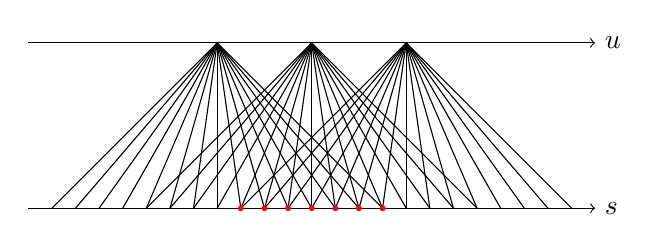
\begin{tikzpicture}[scale = 0.3]
		
		\draw[->] (-9, 0) -- (15, 0);
		\draw[->] (-9, 7) -- (15, 7);
		
		\node[right] at (15, 0) {$s$};
		\node[right] at (15, 7) {$u$};
		
		\draw (-1, 7) -- (-8, 0);
		\draw (-1, 7) -- (-7, 0);
		\draw (-1, 7) -- (-6, 0);
		\draw (-1, 7) -- (-5, 0);
		\draw (-1, 7) -- (-4, 0);
		\draw (-1, 7) -- (-3, 0);
		\draw (-1, 7) -- (-2, 0);
		\draw (-1, 7) -- (-1, 0);
		\draw (-1, 7) -- (0, 0);
		\draw (-1, 7) -- (1, 0);
		\draw (-1, 7) -- (2, 0);
		\draw (-1, 7) -- (3, 0);
		\draw (-1, 7) -- (4, 0);
		\draw (-1, 7) -- (5, 0);
		\draw (-1, 7) -- (6, 0);
		
		\draw (3, 7) -- (-4, 0);
		\draw (3, 7) -- (-3, 0);
		\draw (3, 7) -- (-2, 0);
		\draw (3, 7) -- (-1, 0);
		\draw (3, 7) -- (0, 0);
		\draw (3, 7) -- (1, 0);
		\draw (3, 7) -- (2, 0);
		\draw (3, 7) -- (3, 0);
		\draw (3, 7) -- (4, 0);
		\draw (3, 7) -- (5, 0);
		\draw (3, 7) -- (6, 0);
		\draw (3, 7) -- (7, 0);
		\draw (3, 7) -- (8, 0);
		\draw (3, 7) -- (9, 0);
		\draw (3, 7) -- (10, 0);
		
		\draw (7, 7) -- (0, 0);
		\draw (7, 7) -- (1, 0);
		\draw (7, 7) -- (2, 0);
		\draw (7, 7) -- (3, 0);
		\draw (7, 7) -- (4, 0);
		\draw (7, 7) -- (5, 0);
		\draw (7, 7) -- (6, 0);
		\draw (7, 7) -- (7, 0);
		\draw (7, 7) -- (8, 0);
		\draw (7, 7) -- (9, 0);
		\draw (7, 7) -- (10, 0);
		\draw (7, 7) -- (11, 0);
		\draw (7, 7) -- (12, 0);
		\draw (7, 7) -- (13, 0);
		\draw (7, 7) -- (14, 0);
		
		\draw[fill, red] (0, 0) circle [radius = 0.1];
		\draw[fill, red] (1, 0) circle [radius = 0.1];
		\draw[fill, red] (2, 0) circle [radius = 0.1];
		\draw[fill, red] (3, 0) circle [radius = 0.1];
		\draw[fill, red] (4, 0) circle [radius = 0.1];
		\draw[fill, red] (5, 0) circle [radius = 0.1];
		\draw[fill, red] (6, 0) circle [radius = 0.1];
	\end{tikzpicture}
	
\end{document}
		\label{fig:ShiftedPerspectiveProjection}
	}
	\hfill
	\subfigure[]{
		\centering
		\documentclass{standalone}
\usepackage{tikz}

\begin{document}
	
	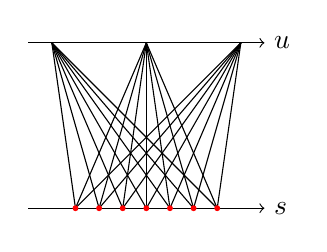
\begin{tikzpicture}[scale = 0.3]
		
		\draw[->] (-2, 0) -- (8, 0);
		\draw[->] (-2, 7) -- (8, 7);
		
		\node[right] at (8, 0) {$s$};
		\node[right] at (8, 7) {$u$};
		
		\draw (-1, 7) -- (0, 0);
		\draw (-1, 7) -- (1, 0);
		\draw (-1, 7) -- (2, 0);
		\draw (-1, 7) -- (3, 0);
		\draw (-1, 7) -- (4, 0);
		\draw (-1, 7) -- (5, 0);
		\draw (-1, 7) -- (6, 0);
		
		\draw (3, 7) -- (0, 0);
		\draw (3, 7) -- (1, 0);
		\draw (3, 7) -- (2, 0);
		\draw (3, 7) -- (3, 0);
		\draw (3, 7) -- (4, 0);
		\draw (3, 7) -- (5, 0);
		\draw (3, 7) -- (6, 0);
		
		\draw (7, 7) -- (0, 0);
		\draw (7, 7) -- (1, 0);
		\draw (7, 7) -- (2, 0);
		\draw (7, 7) -- (3, 0);
		\draw (7, 7) -- (4, 0);
		\draw (7, 7) -- (5, 0);
		\draw (7, 7) -- (6, 0);
		
		\draw[fill, red] (0, 0) circle [radius = 0.1];
		\draw[fill, red] (1, 0) circle [radius = 0.1];
		\draw[fill, red] (2, 0) circle [radius = 0.1];
		\draw[fill, red] (3, 0) circle [radius = 0.1];
		\draw[fill, red] (4, 0) circle [radius = 0.1];
		\draw[fill, red] (5, 0) circle [radius = 0.1];
		\draw[fill, red] (6, 0) circle [radius = 0.1];
		
	\end{tikzpicture}
	
\end{document}
		\label{fig:RectifiedPerspectiveProjection}
	}
	\caption{Perspective projections of a scene. 
			 (a) Projections with three pinhole cameras. 
			 (b) Discarding unused rays corresponds to cropping the camera images.}
\end{figure}


\section{Visualization}
%TODO Show how rectification affects EPI

The epipolar-plane image (EPI) allows for a very intuitive visualization of depth from a 4D light field.
It was first defined by~\cite{EPI} as follows.
Consider a point $P$ in 3D space and a pair of cameras with the optical axis pointing in the same direcion.
The plane passing through $P$ and the two centers of projection is called the \textbf{epipolar plane}.
The epipolar plane projects to a line on each of the camera image planes, named the \textbf{epipolar line}.
This line represents a constraint for the projection of $P$ in each of the images and it is used to solve the correspondance problem in computer vision.
The notion of epipolar lines can be directly applied to a multiple camera setup.
In figure~\ref{fig:epi_example_perspective}, a synthetic scene is rendered in 500 different positions along a horizontal baseline.
Since the camera movement is in horizontal direction only, the epipolar lines correspond to a fixed pixel row in each image.
The EPIs shown in figures~\ref{fig:epi_1x500x1000x1000_scanline1} and ~\ref{fig:epi_1x500x1000x1000_scanline2} are created by collecting the chosen pixel row (scanline) in every image and stacking it up.

The shift in pixels of projections of the same point $P$ in consecutive images is called the (pixel) \textbf{disparity} $D$.
Following the projection of the point $P$ in every image corresponds to a line in the EPI with slope $1 / D$.
\cite{EPI} refer to this line as the \textbf{feature path}.
This means that points farther away from the camera will appear as a feature path in the EPI with steeper slope than points close to the camera.

\begin{figure}[tb]
	\subfigure[]{
		\centering
		\documentclass{standalone}
\usepackage{tikz}
\usepackage{pgfplots}

\begin{document}
	\begin{tikzpicture}[baseline]
		\begin{axis}[	scale only axis,
						height = 2.8cm,
						ylabel near ticks,
						xlabel near ticks, 
						ticks = none, 
						enlargelimits = true, 
						axis on top, 
						axis equal image,
						axis lines = left,
						xlabel = {$x$},
						ylabel = {$y$} 
					]
	
			\addplot graphics [xmin = 0, xmax = 1000, ymin = 0, ymax = 615] {epi_1x500x1000x1000/overview};
		
			\addplot[mark = none, red] coordinates {(0, 615 - 497) (1000, 615 - 497)};
			\addplot[mark = none, red] coordinates {(0, 615 - 236) (1000, 615 - 236)};
			
		\end{axis}
	\end{tikzpicture}	
\end{document}

		\label{fig:epi_1x500x1000x1000_overview}
	}
	\hfill
	\subfigure[]{
		\centering
		\documentclass{standalone}
\usepackage{tikz}
\usepackage{pgfplots}

\begin{document}
	\begin{tikzpicture}[baseline]
		\begin{axis}[	scale only axis,
						height = 2.8cm,
						xtick = {0, 1000}, 
						ytick = {0, 500},
						ylabel near ticks,
						xlabel near ticks, 
						ticks = none, 
						enlargelimits = true, 
						axis on top, 
						axis equal image,
						axis lines = left, 
						xlabel = {$x$}, 
						ylabel = {$u$}
					]
	
			\addplot[plot graphics/node/.append style={yscale=-1,anchor=north west}] % Flip EPI vertically (MATLAB matrix)
					graphics [xmin = 0, xmax = 1000, ymin = 0, ymax = 500] {epi_1x500x1000x1000/scanY=379};
		
		\end{axis}
	\end{tikzpicture}	
\end{document}


		\label{fig:epi_1x500x1000x1000_scanline1}
	}
	\hfill
	\subfigure[]{
		\centering
		\documentclass{standalone}
\usepackage{tikz}
\usepackage{pgfplots}

\begin{document}
	\begin{tikzpicture}[baseline]
		\begin{axis}[	scale only axis,
						height = 2.8cm,
						xtick = {0, 1000}, 
						ytick = {0, 500},
						ylabel near ticks,
						xlabel near ticks, 
						ticks = none, 
						enlargelimits = true, 
						axis on top, 
						axis equal image,
						axis lines = left, 
						xlabel = {$x$}, 
						ylabel = {$u$}
					]
	
			\addplot graphics [xmin = 0, xmax = 1000, ymin = 0, ymax = 500] {epi_1x500x1000x1000/scanY=641};
			
		\end{axis}
	\end{tikzpicture}	
\end{document}
		\label{fig:epi_1x500x1000x1000_scanline2}
	}
	\caption{(a) Raw 3D light field rendered from 500 positions along a horizontal baseline.
				 Two scanlines are extracted from every image. 
			 (b) The feature paths of the blue and green dice have a steeper slope than those of the red die.
			 (c) Feature paths of the yellow die have an even steeper slope, indicating greater depth.}
	\label{fig:epi_example_perspective}
\end{figure}




\section{Light Field Tomography}
%TODO: Derivation according to Wetzstein
% Explain linearity in log domain
% Mention other tomographic projection types
% SART and ART solvers
% Make a chapter?
% Explain "intensity of ray" and unit

The light field display is modeled by a volumetric attenuator $\mu(x, y, z)$ that attenuates the light traveling through its material.
According to the Beer-Lambert law, the intensity of a light ray $\mathcal{R} \subset \mathbb{R}^3$ passing through the material decreases exponentially over distance:
\begin{equation}\label{eq:beer_lambert_law}
	I = I_0 e^{-\int_\mathcal{R} \mu(r) \, \mathrm{d}r }.
\end{equation}
The incident intensity $I_0$ is the intensity of the ray before it enters the attenuator.
Equation~\ref{eq:beer_lambert_law} can be rewritten into 
\begin{equation}\label{eq:log_beer_lambert_law}
	\bar{I} \coloneqq \log \left( \frac{I}{I_0} \right) = -\int_\mathcal{R} \mu(r) \, \mathrm{d}r.
\end{equation} 
Now, let the attenuator $\mu(x, y, z)$ be a cubic slab of height $d$ in Z-direction and let $L(u, v, s, t)$ be the two-plane parameterization of the light field such that the $(s, t)$-plane coincides with the $(x, y)$-plane of the attenuator and the $(u, v)$-plane is at distance $d$.
The set of points describing the ray defined by the coordinates $(u, v, s, t)$ is
\begin{equation}
	\mathcal{R} = \left\{ \lambda a + b 
	\mathrel{\bigg|} a = 
	\begin{pmatrix}
		u - s \\ 
		v - t \\ 
		d
	\end{pmatrix}, 
	b = 
	\begin{pmatrix}
		s \\ 
		t \\ 
		0
	\end{pmatrix},
	\lambda \in \mathbb{R} 
	\right\}.
\end{equation}
A point $p = (x, y, z)^T$ is part of the ray $\mathcal{R}$ if and only if
\begin{align}
	& \exists \lambda \in \mathbb{R} : p = \lambda a + b & & \iff & & a \times (p - b) = 0, 
\end{align} 
where $\times$ denotes the cross product.
Now, $I$ can be replaced with the light field $L$ and the right hand side of equation~\ref{eq:log_beer_lambert_law} can be written as an integral over~$\mathbb{R}^3$:
\begin{equation}\label{eq:log_lightfield_and_radon_transform}
	\bar{L}(u, v, s, t) = 	%\int \limits_{-\infty}^{\infty} \int \limits_{-\infty}^{\infty} \int \limits_{-\infty}^{\infty}
							-\int_{\mathbb{R}^3}
								\mu(p) \delta ( a \times (p - b) ) \, 
							\mathrm{d}p.
\end{equation}
Here, $\delta$ denotes the Dirac delta function on $\mathbb{R}^3$ and $\mu$ is zero outside the boundaries of the slab. 
This means that the integrand is only non-zero for points on the ray with coordinates $(u, v, s, t)$.

Combining equation~\ref{eq:beer_lambert_law} and~\ref{eq:radon_transform} gives the light field emitted by the attenuator.
The goal is to produce such an attenuation display that emits a given target light field.

In computed tomography, the two-dimensional \textbf{radon transform} of a real valued function $f(x, y)$ of compact support is defined as
\begin{equation}
	p(\rho, \theta) = 	\int \limits_{-\infty}^{\infty} 
						\int \limits_{-\infty}^{\infty}
							f(x, y) \delta (x \cos \theta - y \sin \theta - \rho) \, 
						\mathrm{d}x \,
						\mathrm{d}y,
\end{equation}
where $(\rho, \theta) \in \mathbb{R} \times \left(- \frac{\pi}{2}, \frac{\pi}{2}\right)$ defines a ray as shown in figure~\ref{fig:radon_transform_2D_sketch}.
Because the radon transform is essentially a line integral, it can be generalized to three or more dimensions.
Adapting the notation from the two-plane parameterization, the radon transform of the attenuation map $\mu$ along ray $\mathcal{R}$ becomes
\begin{equation}
	p(u, v, s, t) = 	\int \limits_{-\infty}^{\infty} 
						\int \limits_{-\infty}^{\infty}
						\int \limits_{-\infty}^{\infty}
							\mu(x, y, z) \delta \left(a \times \left((x, y, z)^T - b\right) \right) \, 
						\mathrm{d}x \,
						\mathrm{d}y \,
						\mathrm{d}z, 
\end{equation}
which is equivalent to equation~\ref{eq:log_lightfield_and_radon_transform}.
This shows that
\begin{equation}
	\bar{L}(u, v, s, t) = -p(u, v, s, t), 
\end{equation}
or in other words:

\begin{figure}[tb]
	\centering
	\documentclass{standalone}
\usepackage{tikz}
\usetikzlibrary{intersections}

\begin{document}
	
	\begin{tikzpicture}[scale = 0.5]
		
		\draw[->] (-5, 0) -- (5, 0);
		\draw[->] (0, -5) -- (0, 5);
		\node[right] at (5, 0) {$x$};
		\node[above] at (0, 5) {$y$};
		
		\draw plot[smooth cycle] coordinates {(-3, 1) (-2, 2.5) (0, 2) (1.5, 3.5) (2, 2) (2.5, 1) (2, 0) (2, -2) (0.5, -1.5) (-2, -3) (-2, -1)};
		
		\draw[<-] (-1.5, 7.5) -- (-7.5, -1.5); %node[below right] {$\rho$};
		
		\draw[name path = ray, ->] (4, -0.5) -- (-6.5, 6.5);
		\draw (0, 0) -- (-7.5, 5);
		
		\draw (0, 1.5) arc (90 : 180 - atan(2 / 3) : 1.5);
		\node at (-0.4, 0.8) {$\theta$};
		
		\draw[->] (0, 0) -- (1, 1.5) node[pos = 0.4, right] {$\rho$};
		
		\draw[name path = radon] plot[smooth] coordinates {(-6.5, 0) (-6.7, 0.5) (-6.5, 1.2) (-6, 2) (-6.5, 3) (-6, 4.5) (-5, 4.5) (-4, 5.5) (-2.5, 6)};
		
		\fill[name intersections={of= radon and ray, total=\t}]
		\foreach \s in {1,...,\t}{(intersection-\s) circle[radius = 0.1] node[rotate= 90 - atan(2 / 3), above right] {$p(\rho, \theta)$}};
		
		\node[rotate= 90 - atan(2 / 3), right] at (-1.5, 7.5) {$\rho$};
		
	\end{tikzpicture}
	
\end{document}
	\caption{The 2D radon transform of the ray $(\rho, \theta)$ passing a material with density $f(x, y)$.}
	\label{fig:radon_transform_2D_sketch}
\end{figure}


\section{Spectral Analysis}
% Introduction to fourier transform
% Explain the spectral support of LF
% Fourier slice theorem
